\RequirePackage{currfile}
\documentclass[12pt]{beamer}
\usepackage[utf8]{inputenc}
\usepackage[spanish]{babel}
\usepackage{standalone}
\usepackage{color}
\usepackage{siunitx}
\usepackage{hyperref}
%\hypersetup{colorlinks,linkcolor=,urlcolor=blue}
%\hypersetup{colorlinks,urlcolor=blue}
\usepackage{xcolor,soul}
\usepackage{etoolbox}
\usepackage{amsmath}
\usepackage{amsthm}
\usepackage{physics}
\usepackage{multicol}
\usepackage{bookmark}
\usepackage{longtable}
\usepackage{listings}
\usepackage{graphicx}
\usepackage{tikz}
\usetikzlibrary{patterns, matrix, backgrounds, decorations,shapes, arrows.meta}
\usepackage[autostyle,spanish=mexican]{csquotes}
\usepackage[os=win]{menukeys}
\usepackage{pifont}
\usepackage{pbox}
\usepackage{caption}
\captionsetup{font=scriptsize,labelfont=scriptsize}
%\usepackage[sfdefault]{roboto}  %% Option 'sfdefault' only if the base font of the document is to be sans serif

%Sección de definición de colores
\definecolor{ao}{rgb}{0.0, 0.5, 0.0}
\definecolor{bisque}{rgb}{1.0, 0.89, 0.77}
\definecolor{amber}{rgb}{1.0, 0.75, 0.0}
\definecolor{armygreen}{rgb}{0.29, 0.33, 0.13}
\definecolor{alizarin}{rgb}{0.82, 0.1, 0.26}
\definecolor{cadetblue}{rgb}{0.37, 0.62, 0.63}
\definecolor{deepblue}{rgb}{0,0,0.5}
\definecolor{brown}{rgb}{0.59, 0.29, 0.0}
\definecolor{OliveGreen}{rgb}{0,0.25,0}


\usefonttheme[onlymath]{serif}
%Sección de definición de nuevos comandos

\newcommand*{\TitleParbox}[1]{\parbox[c]{1.75cm}{\raggedright #1}}%
\newcommand{\python}{\texttt{python}}
\newcommand{\textoazul}[1]{\textcolor{blue}{#1}}
\newcommand{\azulfuerte}[1]{\textcolor{blue}{\textbf{#1}}}
\newcommand{\funcionazul}[1]{\textcolor{blue}{\textbf{\texttt{#1}}}}
\newcommand{\ptilde}[1]{\ensuremath{{#1}^{\prime}}}
\newcommand{\stilde}[1]{\ensuremath{{#1}^{\prime \prime}}}
\newcommand{\ttilde}[1]{\ensuremath{{#1}^{\prime \prime \prime}}}
\newcommand{\ntilde}[2]{\ensuremath{{#1}^{(#2)}}}
\renewcommand{\arraystretch}{1.5}

\newcounter{saveenumi}
\newcommand{\seti}{\setcounter{saveenumi}{\value{enumi}}}
\newcommand{\conti}{\setcounter{enumi}{\value{saveenumi}}}
\renewcommand{\rmdefault}{cmr}% cmr = Computer Modern Roman

\linespread{1.5}

\usefonttheme{professionalfonts}
%\usefonttheme{serif}
\DeclareGraphicsExtensions{.pdf,.png,.jpg}


%Sección para el tema de beamer, con el theme, usercolortheme y sección de footers
\mode<presentation>
{
  \usetheme{CambridgeUS}
  \setbeamertemplate{headline}{}
  %\useoutertheme{infolines}
  \useoutertheme{default}
  \usecolortheme{rose}
  \setbeamercovered{invisible}
  % or whatever (possibly just delete it)
  \setbeamertemplate{section in toc}[sections numbered]
  \setbeamertemplate{subsection in toc}[subsections numbered]
  \setbeamertemplate{subsection in toc}{\leavevmode\leftskip=3.2em\rlap{\hskip-2em\inserttocsectionnumber.\inserttocsubsectionnumber}\inserttocsubsection\par}
  \setbeamercolor{section in toc}{fg=blue}
  \setbeamercolor{subsection in toc}{fg=blue}
  \setbeamercolor{frametitle}{fg=blue}

  \setbeamertemplate{footline}
  %\beamertemplatenavigationsymbolsempty
}

\makeatletter
\setbeamercolor{section in foot}{bg=gray!30, fg=black!90!orange}
\setbeamercolor{subsection in foot}{bg=blue!30!yellow, fg=red}
\setbeamertemplate{footline}
{
  \leavevmode%
  \hbox{%
  \begin{beamercolorbox}[wd=.333333\paperwidth,ht=2.25ex,dp=1ex,center]{section in foot}%
    \usebeamerfont{section in foot} \insertsection
  \end{beamercolorbox}}%
  \begin{beamercolorbox}[wd=.333333\paperwidth,ht=2.25ex,dp=1ex,center]{subsection in foot}%
    \usebeamerfont{subsection in foot}  \insertsubsection
  \end{beamercolorbox}%
  \begin{beamercolorbox}[wd=.333333\paperwidth,ht=2.25ex,dp=1ex,right]{date in head/foot}%
    \usebeamerfont{date in head/foot} \insertshortdate{} \hspace*{2em}
    \insertframenumber{} / \inserttotalframenumber \hspace*{2ex} 
  \end{beamercolorbox}}%
  \vskip0pt%
\makeatother  

\makeatletter
\patchcmd{\beamer@sectionintoc}
  {\vfill}
  {\vskip\itemsep}
  {}
  {}
\makeatother

% \makeatletter
% \patchcmd{\hyper@link@}
%   {{\Hy@tempb}{#4}}
%   {{\Hy@tempb}{\ul{#4}}}
%   {}{}
% \makeatother


% Sección para el código

\definecolor{Code}{rgb}{0,0,0}
\definecolor{Keywords}{rgb}{255,0,0}
\definecolor{Strings}{rgb}{255,0,255}
\definecolor{Comments}{rgb}{0,0,255}
\definecolor{Numbers}{rgb}{255,128,0}

\DeclareCaptionFont{white}{\color{white}}
\DeclareCaptionFormat{listing}{\colorbox{gray}{\parbox{0.99\textwidth}{#1#2#3}}}
\captionsetup[lstlisting]{format=listing,labelfont=white,textfont=white}
\renewcommand{\lstlistingname}{Código}

\lstset{
basicstyle=\ttfamily,
columns=fullflexible,
breaklines=true
}

\lstdefinestyle{codigopython}{%
  language=Python,                % choose the language of the code
  %basicstyle=\footnotesize\small,       % the size of the fonts that are used for the code
  numbers=left,                   % where to put the line-numbers
  numberstyle=\scriptsize,      % the size of the fonts that are used for the line-numbers
  stepnumber=1,                   % the step between two line-numbers. If it is 1 each line will be numbered
  numbersep=5pt,                  % how far the line-numbers are from the code
  backgroundcolor=\color{white},  % choose the background color. You must add \usepackage{color}
  showspaces=false,               % show spaces adding particular underscores
  showstringspaces=false,         % underline spaces within strings
  showtabs=false,                 % show tabs within strings adding particular underscores
  frame=single,   		% adds a frame around the code
  tabsize=2,  		% sets default tabsize to 2 spaces
  captionpos=t,   		% sets the caption-position to bottom
  breaklines=true,    	% sets automatic line breaking
  breakatwhitespace=false,    % sets if automatic breaks should only happen at whitespace
  escapeinside={\#},  % if you want to add a comment within your code
  stringstyle =\color{OliveGreen},
  texcl = true,
  %otherkeywords={{as}},             % Add keywords here
  keywordstyle = \color{blue},
  commentstyle = \color{black},
  identifierstyle = \color{black},
  % literate=%
  %         {á}{{\'a}}1
  %         {é}{{\'e}}1
  %         {í}{{\'i}}1
  %         {ó}{{\'o}}1
  %         {ú}{{\'u}}1
  %
  %keywordstyle=\ttb\color{deepblue}
  %fancyvrb = true,
literate={0}{{\textcolor{red}{0}}}{1}%
            {1}{{\textcolor{red}{1}}}{1}%
            {2}{{\textcolor{red}{2}}}{1}%
            {3}{{\textcolor{red}{3}}}{1}%
            {4}{{\textcolor{red}{4}}}{1}%
            {5}{{\textcolor{red}{5}}}{1}%
            {6}{{\textcolor{red}{6}}}{1}%
            {7}{{\textcolor{red}{7}}}{1}%
            {8}{{\textcolor{red}{8}}}{1}%
            {9}{{\textcolor{red}{9}}}{1}%
            {.0}{{\textcolor{red}{.0}}}{2}% Following is to ensure that only periods
            {.1}{{\textcolor{red}{.1}}}{2}% followed by a digit are changed.
            {.2}{{\textcolor{red}{.2}}}{2}%
            {.3}{{\textcolor{red}{.3}}}{2}%
            {.4}{{\textcolor{red}{.4}}}{2}%
            {.5}{{\textcolor{red}{.5}}}{2}%
            {.6}{{\textcolor{red}{.6}}}{2}%
            {.7}{{\textcolor{red}{.7}}}{2}%
            {.8}{{\textcolor{red}{.8}}}{2}%
            {.9}{{\textcolor{red}{.9}}}{2}%
            {\ }{{ }}{1}% handle the space
        ,%
        %mathescape=true
        %escapeinside={*@}
        escapeinside={A_}{_B}
}

\title{Tema 3 - Métodos indirectos}
\subtitle{Curso de Física Computacional}
\author[]{M. en C. Gustavo Contreras Mayén}
\date{6 de mayo de 2020}
\begin{document}
\maketitle
\fontsize{14}{14}\selectfont
\spanishdecimal{.}
\section*{Contenido}
\frame[allowframebreaks]{\tableofcontents[currentsection, hideallsubsections]}
\section{Introducción}
\frame{\tableofcontents[currentsection, hideothersubsections]}
\subsection{Motivación}
%Referencia: Newman - Computational physics. 8.6 Boundary value problems
\begin{frame}
\frametitle{Introducción}
Todos el trabajo que hemos considerado hasta este momento han sido sobre EDO con valores iniciales, lo que significa que estamos resolviendo EDO dados los valores iniciales de las variables.
\\
\bigskip
Esta es la forma más común de problema de ecuación diferencial que se encuentra en física, pero no es la única. También hay problemas \emph{con condiciones de frontera o de contorno}.
\end{frame}
\begin{frame}
\frametitle{Introducción}
Considera por ejemplo, la EDO2 que determina la altura sobre el suelo de una pelota lanzada al aire:
\begin{align}
\dv[2]{x}{t} = - g
\label{eq:ecuacion_08_105}
\end{align}
donde $g$ es la aceleración debida a la gravedad e ignoramos la fricción.
\end{frame}
\begin{frame}
\frametitle{Introducción}
Para fijar la solución de esta ecuación, podríamos especificar las condiciones iniciales, siendo necesarias dos condiciones iniciales para una EDO2.
\\
\bigskip
Podríamos por ejemplo, especificar la altura inicial de la pelota y su velocidad inicial hacia arriba. Sin embargo, existe otra posibilidad: podríamos especificar nuestras dos condiciones dando una condición inicial y una condición final.
\end{frame}
\begin{frame}
\frametitle{Introducción}
Por ejemplo, especificar que la pelota tiene una altura $x = 0$ en $t = 0$, luego la altura vuelve a ser $x = 0$ nuevamente en algún momento posterior $t = t_{1}$.
\end{frame}
\begin{frame}
\frametitle{Introducción}
En otras palabras, estamos especificando el momento en que se lanza la pelota y el momento en que cae.
\\
\bigskip
Nuestro objetivo entones, sería encontrar la solución que satisfaga estas condiciones.
\end{frame}
\begin{frame}
\frametitle{Introducción}
Este problema podría surgir, por ejemplo, si quisiéramos calcular la trayectoria de un proyectil necesario para aterrizar en un punto específico, que es un problema clásico en el fuego de artillería (de donde veremos, toma el nombre la primera técnica a revisar).
\\
\bigskip
Los problemas de este tipo se denominan \emph{problemas de condiciones de frontera (CDF) o contorno}.
\end{frame}
\begin{frame}
\frametitle{Problemas tipo CDF}
Los problemas tipo CDF son algo más difíciles de resolver computacionalmente que los problemas de valores iniciales que hemos visto anteriormente, pero se puede lograr una solución combinando técnicas que ya hemos visto.
\end{frame}
\section{El método de disparo}
\frame{\tableofcontents[currentsection, hideothersubsections]}
\subsection{Definición del método}
\begin{frame}
\frametitle{El método de disparo}
Una técnica fundamental para resolver problemas de tipo CDF es el \textoazul{método de disparo}.
\\
\bigskip
El \textoazul{método de disparo} es un \emph{método de ensayo y error} que busca los valores correctos de las condiciones iniciales que coinciden con un conjunto dado de CDF, convirtiendo el cálculo en un problema de valores iniciales.
\end{frame}
\begin{frame}
\frametitle{El método de disparo}
Considera el problema de la pelota mencionado previamente.
\\
\bigskip
En este problema, se nos da la posición inicial pero no la velocidad de la pelota. Todo lo que sabemos es que la pelota cae un cierto tiempo después; la velocidad es lo necesario para que esto suceda.
\end{frame}
\begin{frame}
\frametitle{El método de disparo}
Entonces comenzamos \enquote{adivinando} un valor para la velocidad ascendente inicial.
\\
\bigskip
Usando este valor, resolvemos la ecuación diferencial y seguimos la pelota hasta el tiempo $t_{1}$ en el que se supone que debe aterrizar y nos preguntamos si tenía una altura cero en ese momento.
\end{frame}
\begin{frame}
\frametitle{El método de disparo en una gráfica}
\begin{figure}[h!]
    \centering
    \includestandalone[scale=0.5]{Figuras/metodo_disparo_01}
    \caption{El método de disparo requiere que hagamos la suposición de alguna condición inicial para resolver el problema. En la figura se muestra la trayectoria del lanzamiento de la pelota, en donde debe de aterrizar al tiempo $t = \SI{10}{\second}$.}
\end{figure}
\fontsize{12}{12}\selectfont
Probablemente no fue así. Probablemente sobrepasamos o subestimamos.
\end{frame}
\begin{frame}
\frametitle{Ensayo y error}
En ese caso, cambiamos nuestra estimación de la velocidad inicial e intentamos nuevamente.
\\
\bigskip
La pregunta es \emph{¿cómo exactamente deberíamos modificar nuestras conjeturas para converger al valor correcto para la velocidad inicial?}.
\end{frame}
\begin{frame}
\frametitle{El método de disparo}
Veamos el problema de una manera ligeramente diferente.
\\
\bigskip
En principio, hay alguna función $x = f (v)$ que da la altura $x$ de la pelota en el tiempo $t_{1}$ como una función de la velocidad vertical inicial $v$.
\end{frame}
\begin{frame}
\frametitle{El método de disparo}
No sabemos cuál es esta función, pero podemos calcularla para cualquier valor dado de $v$ resolviendo la ecuación diferencial con esa velocidad inicial.
\\
\bigskip
Nuestro objetivo al resolver el problema de CDF es encontrar el valor de $v$ que hace que la función sea cero.
\end{frame}
\begin{frame}
\frametitle{Primer valor}
Establecemos un primer valor para la velocidad, en la figura anterior para ese valor se tiene la trayectoria $1$, que vemos queda muy corta para alcanzar el punto de aterrizaje a los $10$ segundos.
\end{frame}
\begin{frame}
\frametitle{Segundo valor}
Luego proponemos un segundo valor, que ahora corresponde a la trayectoria $2$ en la gráfica, pero vemos que a los $10$ no ha alcanzado el nivel del suelo, es decir, vamos a quedar muy por delante del punto de aterrizaje.
\end{frame}    
\begin{frame}
\frametitle{Cálculo de una raíz}
Entonces podemos establecer una ecuación tal que $f (v) = 0$.
\\
\bigskip
Pero esto es simplemente una cuestión de encontrar la raíz de la función $f (v)$ y ya sabemos cómo hacerlo, utilizando alguna de las técnicas que vimos en el Tema 2.
\end{frame}
\begin{frame}
\frametitle{Ocupando lo que ya sabemos}
Entonces, el método de disparo implica el uso de uno de los métodos estándar para resolver EDO, como el \textoazul{método Runge-Kutta de cuarto orden (RK4)}, para calcular el valor de la función $f (v)$, que relaciona las condiciones iniciales desconocidas con las  CDF.
\end{frame}
\begin{frame}
\frametitle{El método de disparo}
Luego, usamos un método para calcular la raíz, como el \emph{método de bisección}, para encontrar el valor de esta función, tal que coincida con el valor dado de las CDF.
\end{frame}
\subsection*{Ejemplo: Lanzamiento vertical de una pelota}
\begin{frame}
\frametitle{Ejemplo: Lanzamiento de la pelota}
Planteamos nuevamente el problema del lanzamiento de una pelota que aterriza en el punto $x=0$ después de $10$ segundos.
\end{frame}
\begin{frame}
\frametitle{Primer paso}
Como vimos en las presentaciones anteriores, el primer paso consiste en transformar la EDO2 (ec. \ref{eq:ecuacion_08_105}) a un sistema de dos EDO1:
\begin{align}
\begin{aligned}
\dv{x}{t} &= y \\[0.5em]
\dv{y}{t} &= -g
\end{aligned}
\label{eq:ecuacion_08_106}
\end{align}
\end{frame}
\begin{frame}
\frametitle{Segundo paso}
El siguiente paso es proponer dos valores de velocidad inicial, para luego resolver utilizado \funcionazul{integrate.odeint} con cada valor inicial.
\\
\bigskip
\pause
Una vez obtenidas ambas soluciones, revisamos la manera en determinar la raíz.
\end{frame}
\begin{frame}[fragile]
\frametitle{La función en el código}
Dentro del código la función será entonces:
\begin{lstlisting}[caption=Código para el sistema de dos EDO1, style=codigopython]
def F(y, t):
    F = np.zeros(4, dtype='float64')
    F[0] = y[0]
    F[1] = y[1]
    F[2] = y[3]
    F[3] = -g
    return F
\end{lstlisting}
\end{frame}
\begin{frame}[fragile]
\frametitle{Llamando a \texttt{integrate.odeint}}
El siguiente paso es contar con una función que ocupe \funcionazul{odeint} para resolver el sistema de EDO1 con las condiciones iniciales, la primera que hemos supuesto:
\begin{lstlisting}[caption=Llamando a \texttt{odeint}, style=codigopython]
def velocidad(v, t):
    sol = odeint(F, v, t)
    return sol
\end{lstlisting}
\end{frame}
\begin{frame}[fragile]
\frametitle{Condiciones iniciales y el tiempo}
Falta definir las condiciones iniciales que suponemos, así como la variable temporal:
\begin{lstlisting}[caption=Estableciendo las condiciones iniciales, style=codigopython]
#v = [x, y, dx, dy]

vA_1_B =  [0.0, 0.0, 0.0, 40.0]
vA_2_B =  [0.0, 0.0, 0.0, 60.0]

t = np.linspace(0., 10., 101)
\end{lstlisting}
\end{frame}
\begin{frame}[fragile]
\frametitle{Resolviendo las EDO1}
Se manda llamar la función \funcionazul{odeint} que va a resolver para cada valor de velocidad inicial:
\begin{lstlisting}[caption=Resolviendo el problema para cada condición inicial, style=codigopython]
vA_1_Bcalc = velocidad(vA_1_B, t)
vA_2_Bcalc = velocidad(vA_2_B, t)
\end{lstlisting}
\end{frame}
\begin{frame}[fragile]
\frametitle{Soluciones obtenidas}
Al tomar el último elemento de cada solución:
\begin{verbatim}
valor_v1 = v1calc[:,2][-1]
valor_v2 = v2calc[:,2][-1]
\end{verbatim}
\pause
el valor de velocidad calculada es:
\begin{verbatim}
valor_v1 = -90.50000000008549
valor_v2 = 109.49999999996044
\end{verbatim}
\end{frame}
\begin{frame}[fragile]
\frametitle{Valores con signo contrario}
Encontramos ahora que hay dos valores de velocidad con signos opuestos, por lo que entonces será posible utilizar una técnica para calcular las raíces, tal que $f(v) = 0$:
\begin{verbatim}
f(40) = -90.500
f(60) = 109.499
\end{verbatim}
\end{frame}
\begin{frame}
\frametitle{Gráfica obtenida}
Incorporamos una rutina de graficación y la correspondiente función para describir la trayectoria de la pelota (recordando lo que aprendimos en el curso de Mécanica vectorial) para cada velocidad inicial propuesta:
\end{frame}
\begin{frame}
\frametitle{Gráfica obtenida}
\begin{figure}[h!]
    \centering
    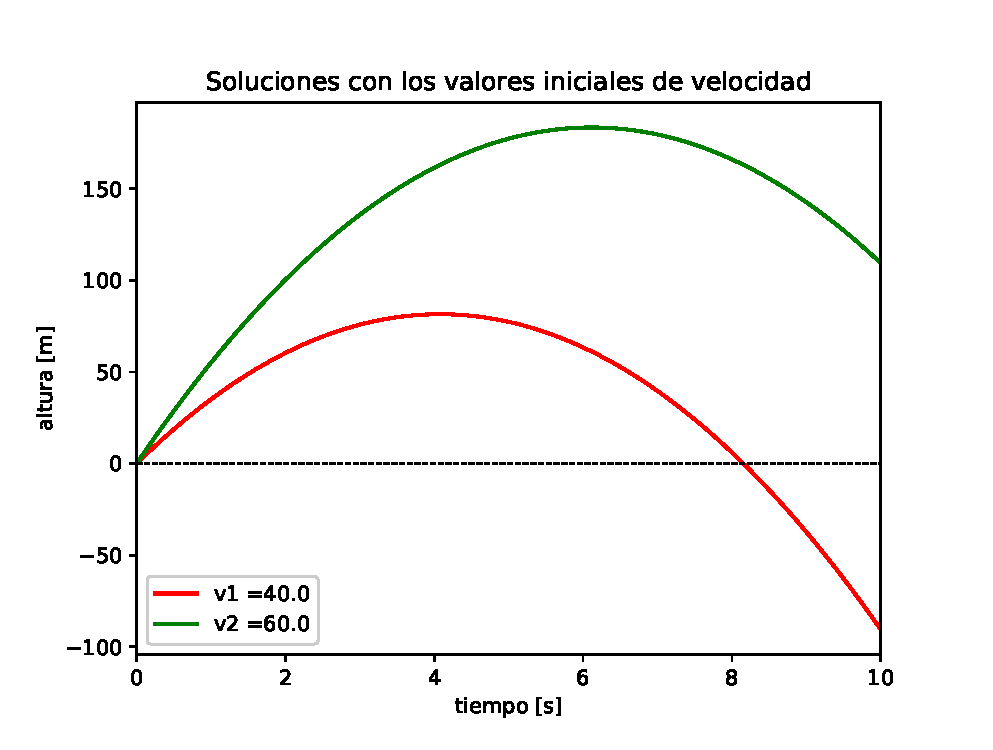
\includegraphics[scale=0.55]{Imagenes/metodo_disparo_2020_01.eps}
\end{figure}
\end{frame}
\begin{frame}
\frametitle{Gráfica obtenida}
Utilizando los valores de velocidad propuestos y con \funcionazul{odeint}, tenemos que para la velocidad $v_{1} = \SI{40}{\meter\per\second}$ la pelota aterrizó antes de los $\SI{10}{\meter}$, mientras que para la $v_{2} = \SI{60}{\meter\per\second}$ la pelota no aterriza a los $\SI{10}{\meter}$, sino que continua su trayectoria.
\end{frame}
\begin{frame}
\frametitle{Sobre la técnica para obtener la raíz}
En el Tema 2, revisamos varias técnicas para obtener una raíz, a partir de una función explícita, es decir, conocemos como tal la función, y podríamos usar alguna de las técnicas referidas.
\\
\bigskip
Veamos una propiedad de la EDO2 inicial y su utilidad para simplificar el cálculo del valor buscado.
\end{frame}
\begin{frame}
\frametitle{EDO2 lineal}
Si tenemos una EDO2 lineal, los valores obtenidos por el sistema de dos EDO1 están relacionados linealmente, de tal manera que podemos utilizar una interpolación lineal para calcular el valor de velocidad.
\end{frame}
\begin{frame}[fragile]
\frametitle{Uso de interpolación}
Ahora aprovechamos el uso de la función de interpolación que está incluida en el paquete \funcionazul{numpy}:
\begin{verbatim}
vn = [v1[3], v2[3]]
hn = [valor_v1, valor_v2]

ajuste = np.interp(0.0, hn, vn)
print("La velocidad inicial que se requiere 
    es {0:1.10f} m/s".format(ajuste))
\end{verbatim}
\end{frame}
\begin{frame}
\frametitle{Valor de velocidad obtenido}
El valor que obtenemos a partir de la inteporlación es $v = \SI{49.05}{\meter\per\second}$, tal que al incluirlo en la rutina de graficación, vemos que resuelve la EDO2 con las condiciones de altura de la pelota en los tiempos $t = 0$ y $t = 10$:
\end{frame}
\begin{frame}
\frametitle{Gráfica obtenida con la velocidad}
\begin{figure}[h!]
    \centering
    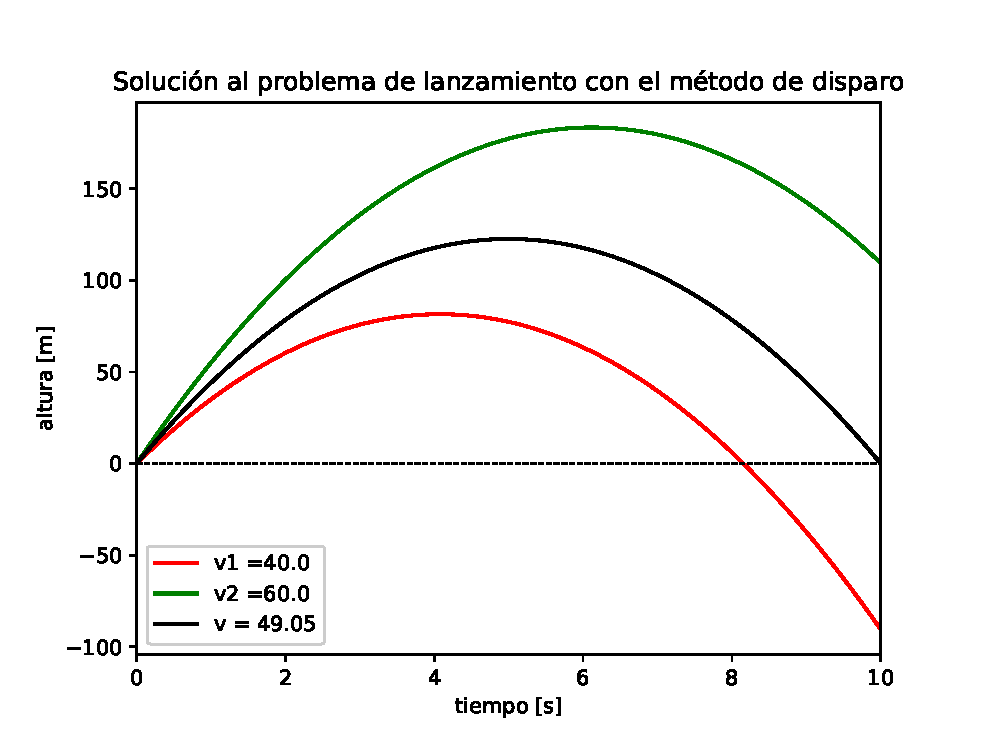
\includegraphics[scale=0.55]{Imagenes/metodo_disparo_2020_02.eps}
\end{figure}
\end{frame}
\begin{frame}
\frametitle{Ejercicio a cuenta}
Se presentó por bloques el código que resuelve este problema, ahora te toca reunir todos los elementos para reproducir las soluciones y gráficas obtenidas, en un sólo código de \python.
\end{frame}
\begin{frame}
\frametitle{Ejercicio a cuenta}
Resolviendo con integración numérica al problema de valores iniciales:
\begin{align*}
\stilde{y} + \ptilde{y} - y = 0, \hspace{0.5cm} y(0) = 0, \hspace{0.5cm} \ptilde{y}(0) = 1
\end{align*}
obtenemos que $y(1) = 0.741028$. 
\\
\bigskip
¿Qué valor deberá tener $\ptilde{y}(0)$ que resultaría en $y(1) = 1$, suponiendo que $y(0)$ no cambia?
\end{frame}
\section{Método de diferencias finitas}
\frame{\tableofcontents[currentsection, hideothersubsections]}
\subsection{Generalidades del método}
\begin{frame}
\frametitle{El método de diferencias finitas}
El \textoazul{método de disparo} tiene problemas de redondeo cuando una de las soluciones es
una exponencial creciente que crece demasiado deprisa
\\
\bigskip
El \textoazul{método de diferencias finitas} tiene un mejor comportamiento en este aspecto, pero \emph{requiere un mayor tiempo de cálculo}.
\end{frame}
\begin{frame}
\frametitle{El método de diferencias finitas}
En el \textoazul{método de diferencias finitas}, dividimos el rango de integración $(a, b)$ en $m$ subintervalos iguales de longitud $h$ cada uno, como se muestra en la siguiente figura.
\end{frame}
\begin{frame}
\frametitle{El método de diferencias finitas}
\begin{figure}[h!]
    \centering
    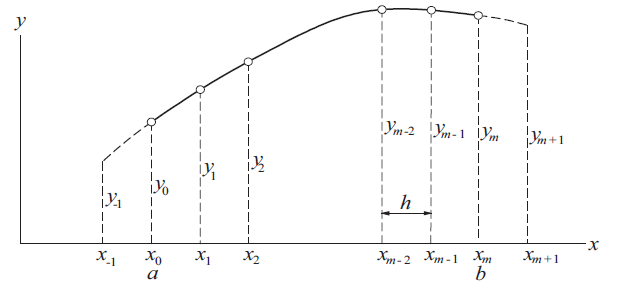
\includegraphics[scale=0.6]{Imagenes/metodo_diferencias_finitas_01.png}
    \caption{Malla de integración para el método de diferencias finitas.}
\end{figure}
\end{frame}
\begin{frame}
\frametitle{El método de diferencias finitas}
Los valores de la solución numérica en los puntos de la malla se denotan por $y_{i}, i = 0, 1, \ldots, m$
\\
\bigskip
El propósito de incluir $y_{-1}$ y $y_{m+ 1}$ se explicará en breve.
\end{frame}
\begin{frame}
\frametitle{Dos aproximaciones}
Entonces se realizan dos aproximaciones:
\setbeamercolor{item projected}{bg=blue!70!black,fg=yellow}
\setbeamertemplate{enumerate items}[circle]
\begin{enumerate}[<+->]
\item Las derivadas de $y$ en la EDO se reemplazan por las expresiones de diferencias finitas que revisamos en el Tema 2.
\seti
\end{enumerate}
\end{frame}
\begin{frame}
\frametitle{Dos aproximaciones}
\setbeamercolor{item projected}{bg=blue!70!black,fg=yellow}
\setbeamertemplate{enumerate items}[circle]
\begin{enumerate}[<+->]
\conti
\item Las EDO se resuelve solo en los puntos de la malla.
\end{enumerate}
\end{frame}
\begin{frame}
\frametitle{Resultado del método}
Como resultado, las ecuaciones diferenciales se reemplazan por un sistema de $m+1$ ecuaciones algebraicas simultáneas, siendo las incógnitas $y_{i}, i = 0, 1, \ldots, m$. 
\\
\bigskip
Si la ED no es lineal, las ecuaciones algebraicas también serán no lineales y deberán resolverse mediante el \textoazul{método de Newton-Raphson}.
\end{frame}
\begin{frame}
\frametitle{Resultado del método}
Dado que el error de truncamiento en una primera aproximación de diferencias centrale es del orden de $\order{h^{2}}$, el \textoazul{método de diferencias finitas} \emph{no es tan preciso} como el \textoazul{método de disparo}; recordemos que el \textoazul{método Runge-Kutta} tiene un error de truncamiento de $\order{h^{5}}$.
\end{frame}
\subsection{Construyendo el método}
\begin{frame}
\frametitle{La EDO2 lineal}
Una EDO2 lineal no homogénea con coeficientes variables, es de la forma
\begin{align}
\dv[2]{y(x)}{x} + p(x) \, \dv{y(x)}{x} + q(x) \, y(x) =  f(x)
\label{eq:ecuacion_01}
\end{align}
donde $p(x)$ y $q(x)$ son coeficientes variables.
\end{frame}
\begin{frame}
\frametitle{Construyendo el método}
Para establecer el método numérico, primeramente se \emph{aproximan la primera y segunda derivadas} de una función generalizada $y(t)$ a partir del desarrollo en series de Taylor alrededor de un punto $t=x+h$ y $t=x-h$, esto es:
\end{frame}
\begin{frame}
\frametitle{Aproximación de la primera derivada}
Esta operación ya la realizamos en el Tema 2, y encontramos que
\begin{align}
y(x+h) - y(x-h) =  2 \, h \, \ptilde{y} (x)
\label{eq:ecuacion_05}
\end{align}
\pause
Renombrando $y(x+h) = y_{i+1}$ así como  $y(x-h)=y_{i-1}$, se obtiene la aproximación de la primera derivada
\begin{align}
\ptilde{y} (x) \approx \dfrac{y_{i+1} - y_{i-1}}{2 \, h}
\label{eq:ecuacion_06}
\end{align}
\end{frame}
\begin{frame}
\frametitle{Aproxmación segunda derivada}
Para la segunda derivada tenemos que
\begin{align}
y(x+h) + y(x-h) = 2 \, y(x) + \stilde{y} (x) \, h^{2}
\label{eq:ecuacion_07}
\end{align}
\pause
renombrando $y(x+h) = y_{i+1}$,  $y(x-h)=y_{i-1}$, $y(x) = y_{i}$, obtenemos la expresión de la segunda derivada
\begin{align}
\stilde{y}(x) \approx \dfrac{y_{i+1} - 2 \, y_{i} + y_{i-1}}{h^{2}}
\label{eq:ecuacion_08}
\end{align}
\end{frame}
\begin{frame}
\frametitle{Reescribiendo la EDO2}
Al sustituir $y(x)=y_{i}$, además de las ecs. (\ref{eq:ecuacion_06}) y (\ref{eq:ecuacion_08}), en la EDO2 (ec. \ref{eq:ecuacion_01}), tenemos
\fontsize{12}{12}\selectfont
\begin{align}
\dfrac{y_{i+1} - 2 \, y_{i} + y_{i-1}}{h^{2}} + p(x) \, \left( \dfrac{y_{i+1} - y_{i-1}}{2 \, h}  \right) + q(x) \, y_{i} = f(x)
\label{eq:ecuacion_09}
\end{align}
\end{frame}
\begin{frame}
\frametitle{Reescribiendo la EDO2}
Ahora renombramos $p(x) = p_{i}$, $q(x) = q_{i}$ y $f(x) = f_{i}$, para luego sumar términos semejantes y obtenemos la expresión:
\begin{align}
\begin{aligned}
y_{i-1} \left( 1- \dfrac{h}{2} \, p_{i} \right) &+ y_{i} \left( q_{i} \, h^{2} -2 \right) + \\[0.5em]
&+ y_{i+1} \left( 1 + \dfrac{h}{2} \, p_{i} \right) = h^{2} \, f_{i}
\end{aligned}
\label{eq:ecuacion_10}
\end{align}
\end{frame}
\begin{frame}
\frametitle{Reexpresión matricial}
Dado que los coeficientes de las funciones $y$ forman parte de una matriz, se nombran de la siguente manera: $a_{i, j-1}$, $a_{i,j}$ $a_{i, j+1}$, para recuperar la expresión
\begin{align}
y_{i-1} \, \big( a_{i, j-1} \big) + y_{i} \, \big( a_{i, j} \big) + y_{i+1} \, \big( a_{i, j+1} \big) = h^{2} \, f_{i}
\label{eq:ecuacion_11}
\end{align}
\end{frame}
\begin{frame}
\frametitle{Matriz de coeficientes}
En donde
\begin{align}
a_{i, j-1} &= 1 -\dfrac{h}{2} \, p_{i} \label{eq:ecuacion_12} \\[0.5em]
a_{i, j} &= q_{i} \, h^{2} - 2 \label{eq:ecuacion_13} \\[0.5em]
a_{i, j+1} &= 1 +\dfrac{h}{2} \, p_{i} \label{eq:ecuacion_14}
\end{align}
\end{frame}
\begin{frame}
\frametitle{Una buena aproximación}
Obtener una buena aproximación a la solución exacta de la ED depende del tamaño del paso $h$ , pero éste, está relacionado con el factor  $q_{i}$, ya que forma parte de la diagonal principal de la matriz de coeficientes que se forma y que está expresado en la ec. (\ref{eq:ecuacion_13}).
\end{frame}
\begin{frame}
\frametitle{Valor de paso máximo}
Haciendo que la ec. (\ref{eq:ecuacion_13}) sea menor que cero, se obtiene el tamaño de paso máximo, es decir
\begin{align}
q_{i} \, h^{2} - 2 < 0 \hspace{0.25cm} \Rightarrow \hspace{0.25cm} h < \sqrt{\dfrac{2}{q_{i}}}
\label{eq:ecuacion_15}
\end{align}
\end{frame}
\begin{frame}
\frametitle{Número mínimo de pasos}
Por lo que el número mínimo $N$ de pasos de cálculo se expresa como:
\begin{align}
N = \dfrac{b - a}{h} \hspace{0.25cm} \Rightarrow \hspace{0.25cm} N = (b - a) \sqrt{\dfrac{q_{i}}{2}}
\label{eq:ecuacion_16}
\end{align}
\end{frame}
\begin{frame}
\frametitle{Valor de $N$}
Para fines prácticos, el \emph{número de pasos es de 3 ó 4} veces este valor mínimo de $N$ , ya que para un número de pasos cercano a $N$ , se tiene un mal ajuste de la solución de la EDO.
\end{frame}
\begin{frame}
\frametitle{Valor de $N$}
Para aplicar el \textoazul{método de diferencias finitas} a una ED se debe tener en cuenta que los
valores de la función $y(x)$ en los extremos del intervalo $[a,b]$ son respectivamente $y(a) = y_{0}$ y $y(b) = y_{N}$, por lo que el primer valor a evaluar es para $i = 1$ y el último es para $i = N - 1$.
\end{frame}
\begin{frame}
\frametitle{Sistema de ecuaciones algebraicas}
Dado que para cada valor de $i$ se tiene una ecuación lineal, el problema de resolver una ED se ha convertido en darle solución a un sistema de $N - 1$ ecuaciones algebraicas con $N - 1$ incógnitas.
\end{frame}
\begin{frame}
\frametitle{Técnicas de solución}
Como es sabido, determinar las soluciones de un sistema de ecuaciones algebraicas se puede obtener usando por ejemplo el \textoazul{método de Gauss-Jordan}.
\end{frame}
\subsection{Ejemplo del método}
\begin{frame}
\frametitle{Ejemplo del método}
Usando el \textoazul{método de diferencias finitas} resolvermos una ED que se obtiene de un sistema mecánico de masa-resorte, es decir, de un problema de mecánica.
\end{frame}
\begin{frame}
\frametitle{El problema}
Una masa de $6$ libras estira un resorte que mide $6$ pulgadas, hay una fuerza de amortiguamiento tal que es $1.5$ veces la velocidad instantánea que actúa sobre el resorte.
\\
\bigskip
\pause
Si se desplaza a la masa $4$ pulgadas por debajo de su posición de equilibrio y se libera, \emph{encuentra:} a) la EDO para el resorte, b) la solución a la EDO mediante el método de diferencias finitas.
\end{frame}
\begin{frame}
\frametitle{Construyendo la EDO}
Obtenemos la constante $k$ del resorte a partir de la ley de Hooke:
\begin{align}
W = k \, x
\end{align}
\end{frame}
\begin{frame}
\frametitle{Construyendo la EDO}
A partir de la segunda ley de Newton, tenemos la primera respuesta, es decir, la EDO2 con coeficientes constantes:
\begin{align}
\left( \dfrac{6}{32} \right) \dv[2]{y}{t} = -1.5 \dv{y}{t} - 12 \, y
\label{eq:ecuacion_18}
\end{align}
Las condiciones iniciales en $t = 0$, son:
\begin{align*}
x = \dfrac{1}{3} \hspace{1cm} \ptilde{y} = 0
\end{align*}
\end{frame}
\begin{frame}
\frametitle{Solución exacta de la EDO}
Vamos a ocupar la solución exacta de la EDO, así que se presenta a continuación:
\begin{align}
y = \dfrac{2 \, \sqrt{3}}{9} \exp(-4 \, t) \, \sin \left( 4 \, \sqrt{3} + \dfrac{\pi}{3}\right)
\label{eq:ecuacion_19}
\end{align}
Sería un buen ejercicio que obtuvieras a mano la solución, y no sustituirla en la EDO2 para demostrar que es solución.
\end{frame}
\begin{frame}
\frametitle{Expresar a modo la EDO2 obtenida}
La EDO2 dada en la ec. (\ref{eq:ecuacion_18}) debe de ser expresada en la forma del modelo de solución, es decir, de la manera en la ec. (\ref{eq:ecuacion_01}), por lo que:
\begin{align}
\dv[2]{y}{t} + 8 \, \dv{y}{t} + 64 \, y = 0
\label{eq:ecuacion_20}
\end{align}
entonces se tiene:
\begin{align}
p(x) &= 8 \label{eq:ecuacion_21} \\
q(x) &= 64 \label{eq:ecuacion_22} \\
f(x) &= 0 \label{eq:ecuacion_23}
\end{align}
\end{frame}
\begin{frame}
\frametitle{Primera ejecución}
Para ver la operación del método, se realizará una primera ejecución de $5$ pasos (valor que es menor a la $N$ mínima calculada con la ec. (\ref{eq:ecuacion_16}), que sería de $N = 6$.
\end{frame}
\begin{frame}
\frametitle{El valor de $h$}
Entonces el tamaño de $h$ (distancia entre cada punto de la malla) es
\begin{align*}
h = \dfrac{b - a}{N} = \dfrac{1}{5} = 0.2
\end{align*}
\end{frame}
\begin{frame}
\frametitle{Valores en las fronteras}
Los valores de frontera son
\begin{align*}
y_{0} (t=0) = \dfrac{1}{3} \hspace{1cm} y_{5}(1) = 0.007
\end{align*}
que se calcularon a partir de la ec. (\ref{eq:ecuacion_19}). Estos valores son los datos iniciales del problema. Para aplicar el método, en este caso, los tomamos de una evaluación directa a la solución de la EDO.
\end{frame}
\begin{frame}
\frametitle{Valores de los coeficientes}
Al ser $p(x)$ y $q(x)$ constantes, los valores de
\begin{align*}
a_{i,j-1} &= 0.2 \\[0.25em]
a_{i,j} &= 0.56 \\[0.25em]
a_{i,j+1} &= 1.8
\end{align*}
también son constantes.
\end{frame}
\begin{frame}
\frametitle{Sistema de ecuaciones algebraicas}
Comenzando con $N = 1$ se construye el sistema de ecuaciones de donde se obtendrá una matriz tridiagonal.
\begin{align}
0.2 \, y_{0} + 0.56 \, y_{1} + 1.8 \, y_{2} &= 0 \label{eq:ecuacion_24} \\[0.25em]
0.2 \, y_{1} + 0.56 \, y_{2} + 1.8 \, y_{3} &= 0 \label{eq:ecuacion_25} \\[0.25em]
0.2 \, y_{2} + 0.56 \, y_{3} + 1.8 \, y_{4} &= 0 \label{eq:ecuacion_26} \\[0.25em]
0.2 \, y_{3} + 0.56 \, y_{4} + 1.8 \, y_{5} &= 0 \label{eq:ecuacion_27}
\end{align}
\fontsize{12}{12}\selectfont
donde $y_{0}$ y $y_{5}$ son los valores de CDF, que deben de multiplicarse por $a_{1,0}$ y $a_{4,5}$, respectivamente.
\end{frame}
\begin{frame}
\frametitle{Sistema de ecuaciones obtenido}
Reescribiendo estos valores al otro lado de la igualdad, obtenemos un sistema de ecuaciones, que expresado en forma de matrices es:
\begin{align*}
\begin{bmatrix}
0.56 & 1.8 & 0 & 0 \\
0.2 & 0.56 & 1.8 & 0 \\
0 & 0.2 & 0.56 & 1.8 \\
0 & 0 & 0.2 & 0.56
\end{bmatrix}
\begin{bmatrix}
y_{1} \\
y_{2} \\
y_{3} \\
y_{4}
\end{bmatrix} =
\begin{bmatrix}
-0.0667 \\
0 \\
0 \\
-0.0126
\end{bmatrix}
\end{align*}
\end{frame}
\begin{frame}
\frametitle{Sobre el sistema de ecuaciones}
En el sistema de ecuaciones obtenido se forma una \emph{matriz tridiagonal}. En álgebra lineal las matrices triangulares tienen una serie de propiedades y métodos de solución, dependiendo si son simétricas o no, si todos los elementos son no nulos, etc.
\\
\bigskip
Este sistema se resuelve utilizando el método de la matriz ampliada con una \textoazul{reducción de Gauss-Jordan}.
\end{frame}
\begin{frame}
\frametitle{Solución al sistema de ecuaciones}
En este punto haremos un \enquote{adelanto} en cuanto a mostrar las soluciones del sistema obtenido, ya que en el Tema 4 del curso, nos enfocaremos al estudio computacional de matrices, técnicas de solución. Sería un buen momento para repasar lo aprendido del curso de Álgebra Lineal 1.
\end{frame}
\begin{frame}
\frametitle{Solución sistema de ecuaciones}
En la siguiente tabla, se muestra el resultado al resolver el sistema de ecuaciones. Donde en la primer columna se tiene el número de pasos $N$, la segunda columna los valores que va tomado $x$ (puntos en la malla), en la tercera columna se tienen los valores de $y$ evaluados (en la solución exacta) y en la última columna los valores calculados.
\end{frame}
\begin{frame}
\frametitle{Solución sistema de ecuaciones}
\fontsize{12}{12}\selectfont
\begin{table}
\begin{tabular}{| c | c | c | c | } \hline
$N$ & $x_{i}$ & $y(x)$ & $y_{i}$ \\\hline
$0$ & $0$ & $0.3333$ & $0.3333$ \\\hline
$1$ & $0.2$ & $-0.0487$ & $-0.8000$ \\\hline
$2$ & $0.4$ & $-0.0487$ & $0.2120$ \\\hline
$3$ & $0.6$ & $-0.0308$ & $0.0229$ \\\hline
$4$ & $0.8$ & $0.0047$ & $0.0307$ \\\hline
$5$ & $1.0$ & $0.0070$ & $0.0070$ \\\hline
\end{tabular}
\end{table}
\end{frame}
\begin{frame}
\frametitle{Gráfica de los resultados}
En la siguiente figura se presentan las gráficas a partir de los puntos mostrados en la tabla anterior, es decir, la gráfica de la solución exacta (con $5$ puntos) en color rojo, y la gráfica de la solución (la aproximación) en color azul.
\end{frame}
\begin{frame}
\frametitle{Gráfica de los resultados}
\begin{figure}[h!]
    \centering
    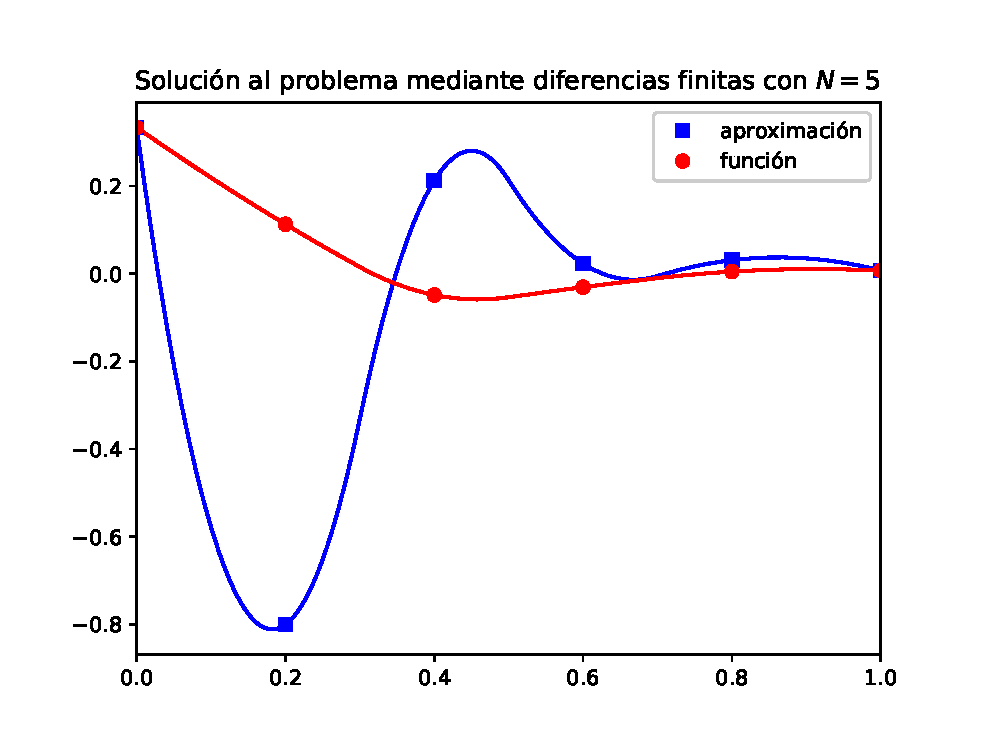
\includegraphics[scale=0.5]{Imagenes/metodo_diferencias_finitas_02.eps}
    \caption{Solución obtenida al resolver el sistema de ecuaciones con $N=5$.}
\end{figure}
\end{frame}
\begin{frame}
\frametitle{Resultado obtenido}
De la gráfica vemos que al tomar un valor de $N = 5$ que es menor que al mínimo dado por la ec. (\ref{eq:ecuacion_16}), la solución numérica no se aproxima a la solución exacta.
\end{frame}
\begin{frame}
\frametitle{Incremento en el valor de $N$}
Incrementamos el valor de $N$, siendo ahora $N=6$  que es el valor mínimo que se obtuvo en la ec. (\ref{eq:ecuacion_16}).
\\
\bigskip
Al volver a calcular los valores de los coeficientes, tenemos que:
\end{frame}
\begin{frame}
\frametitle{Valores de los coeficientes}
Con $N = 6$, los coeficientes tienen el valor
\begin{align*}
a_{i, j-1} = 0.3333, \hspace{0.25cm} a_{i, j} = -0.2222, \hspace{0.25cm} a_{i, j+1} = 1.6667
\end{align*}
Entonces ahora tendremos una matriz de tamaño $5 \times 5$, que se muestra a continuación y  deberemos de resolver:
\end{frame}
\begin{frame}
\frametitle{Valores de los coeficientes}
\fontsize{10}{10}\selectfont
\begin{align*}
\begin{bmatrix}
-0.2222 & 1.6667 & 0 & 0 & 0 \\
0.3333 & -0.2222 & 1.6667 & 0 & 0 \\
0 & 0.3333 & -0.2222 & 1.6667 & 0 \\
0 & 0 & 0.3333 & -0.2222 & 1.6667 \\
0 & 0 & 0 & 0.3333 & -0.2222
\end{bmatrix}
\begin{bmatrix}
y_{1} \\
y_{2} \\
y_{3} \\
y_{4} \\
y_{5}
\end{bmatrix} =
\begin{bmatrix}
-0.1111 \\
0 \\
0 \\
0 \\
-0.0117
\end{bmatrix}
\end{align*}
\end{frame}
\begin{frame}
\frametitle{Resultdos para $N=6$}
De forma similar se presentan los valores obtenidos al resolver este último sistema de ecuaciones, se
muestran en la siguiente tabla.
\end{frame}
\begin{frame}
\frametitle{Solución sistema de ecuaciones $N=6$}
\fontsize{10}{10}\selectfont
\begin{table}
\begin{tabular}{| c | c | c | c | } \hline
$N$ & $x_{i}$ & $y(x)$ & $y_{i}$ \\\hline
$0$ & $0$ & $0.3333$ & $0.3333$ \\\hline
$1$ & $0.1666$ & $0.1595$ & $0.6361$ \\\hline
$2$ & $0.3333$ & $-0.0216$ & $0.0181$ \\\hline
$3$ & $0.5$ & $-0.0510$ & $-0.1247$ \\\hline
$4$ & $0.6667$ & $-0.0155$ & $-0.0202$ \\\hline
$5$ & $0.8333$ & $0.0070$ & $0.0222$ \\\hline
$6$ & $1.0000$ & $0.0070$ & $0.0070$ \\\hline
\end{tabular}
\end{table}
\end{frame}
\begin{frame}
\frametitle{Gráfica de los resultados $N=6$}
\begin{figure}[h!]
    \centering
    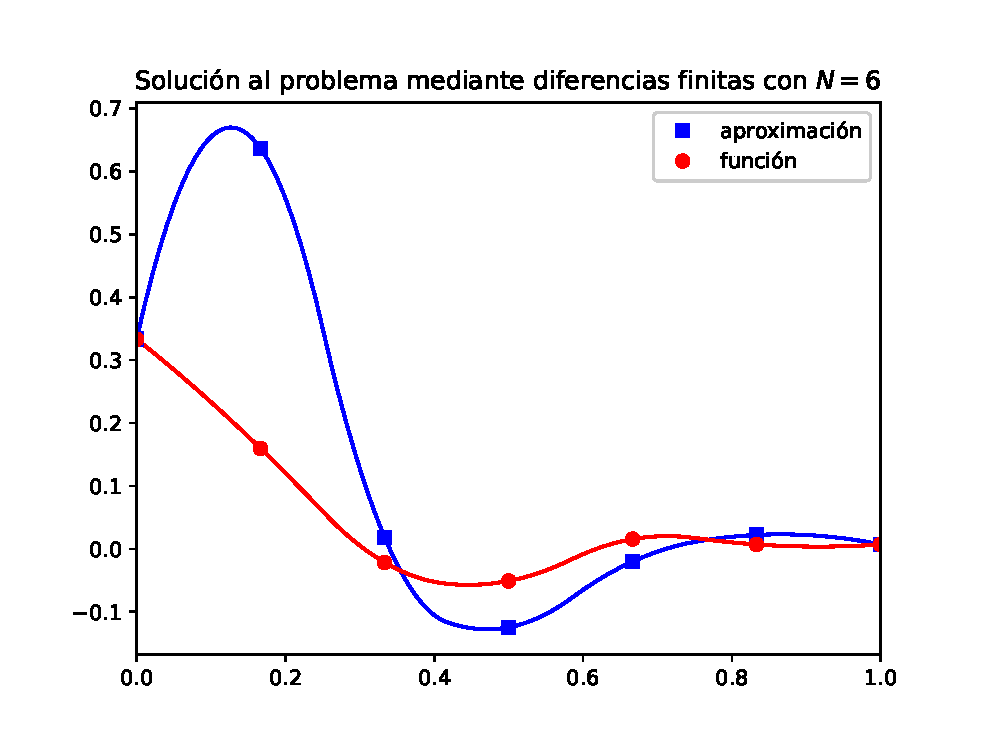
\includegraphics[scale=0.5]{Imagenes/metodo_diferencias_finitas_03.eps}
    \caption{Solución obtenida al resolver el sistema de ecuaciones con $N=6$.}
\end{figure}
\end{frame}
\begin{frame}
\frametitle{Resultado obtenido con $N=6$}
En la nueva gráfica se observa que aún cuando $N$ toma el valor mínimo $(N = 6)$, no se obtiene un ajuste adecuado a la solución algebraica.
\\
\bigskip
El siguiente paso natural sería incrementar de manera unitaria el valor de $N$, pero haremos un \enquote{brinco} y pasaremos a $N=8$
\end{frame}
\begin{frame}
\frametitle{Coeficientes para $N=8$}
Nuevamente se calculan los coeficientes, se obtiene así un sistema de $7 \times 7$ ecuaciones con $7$ incógnitas, que se resuelve nuevamente con el \textoazul{método de Gauss-Jordan}.
\end{frame}
\begin{frame}
\frametitle{Gráfica de los resultados $N=8$}
\begin{figure}[h!]
    \centering
    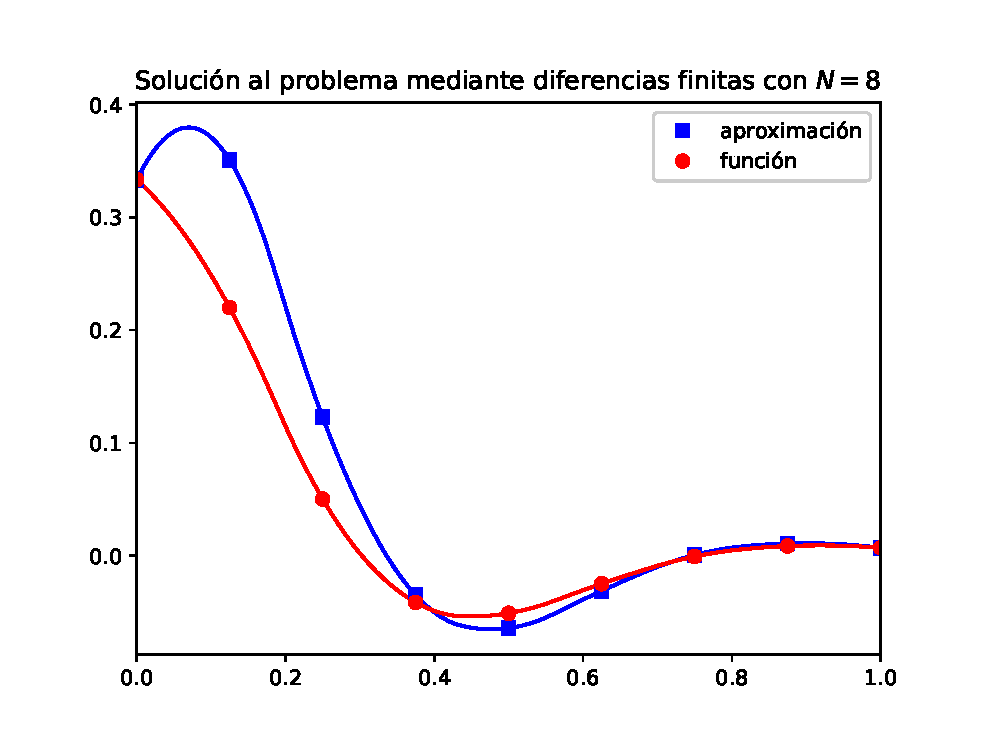
\includegraphics[scale=0.5]{Imagenes/metodo_diferencias_finitas_04.eps}
    \caption{Solución obtenida al resolver el sistema de ecuaciones con $N=8$.}
\end{figure}
\end{frame}
\begin{frame}
\frametitle{Resultado obtenido con $N=8$}
En la nueva gráfica se observa que no se obtiene un ajuste adecuado a la solución algebraica, aunque ya va mejorando, pero no podemos dar por hecho que las soluciones coinciden.
\\
\bigskip
\pause
A continuación se presentan las gráficas obtenidas para $N=10$ y $N=20$. (Resolver estos sistemas algebraicos a mano, sería muy tedioso ¿cómo le harías para automatizar las cuentas?)
\end{frame}
\begin{frame}
\frametitle{Gráfica de los resultados $N=10$}
\begin{figure}[h!]
    \centering
    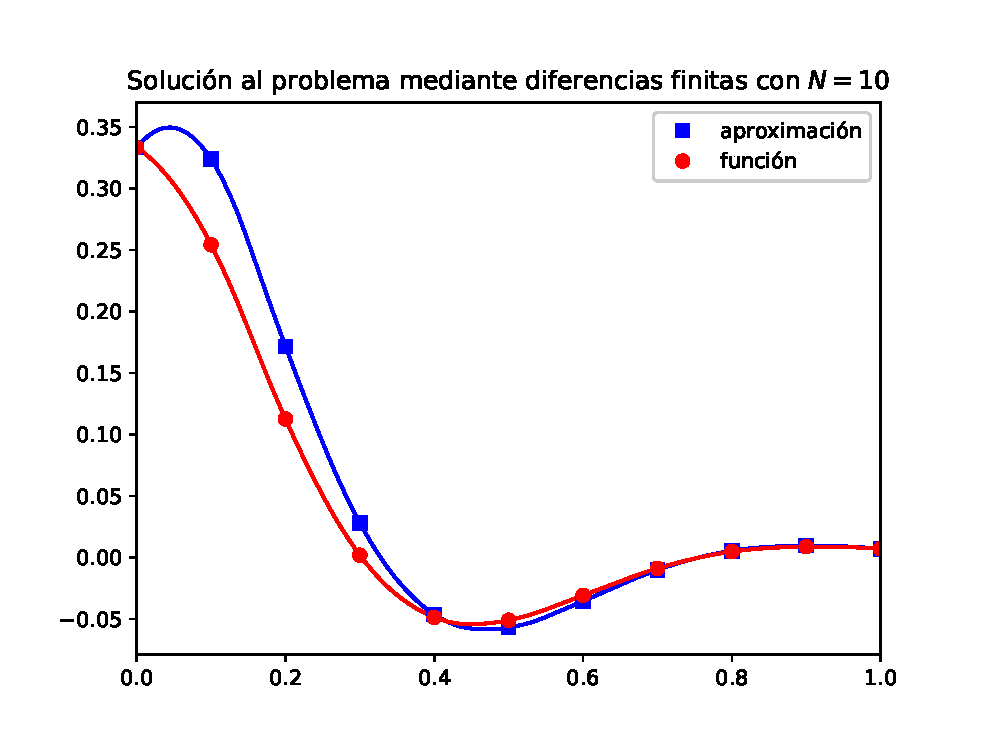
\includegraphics[scale=0.5]{Imagenes/metodo_diferencias_finitas_05.eps}
    \caption{Solución obtenida al resolver el sistema de ecuaciones con $N=10$.}
\end{figure}
\end{frame}
\begin{frame}
\frametitle{Gráfica de los resultados $N=20$}
\begin{figure}[h!]
    \centering
    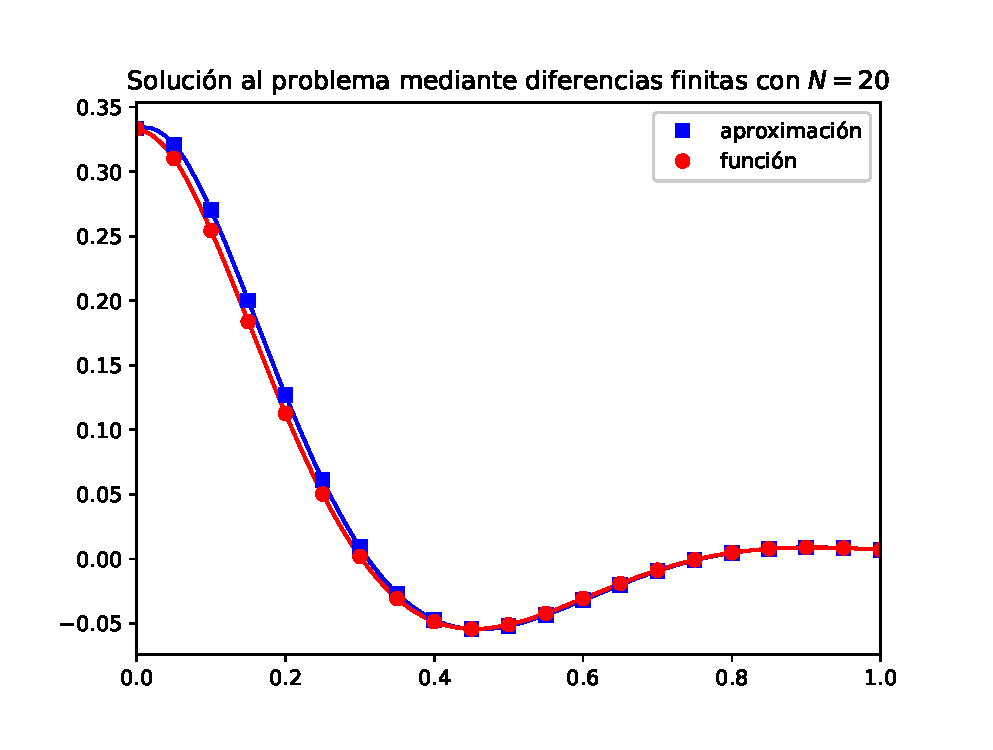
\includegraphics[scale=0.5]{Imagenes/metodo_diferencias_finitas_06.eps}
    \caption{Solución obtenida al resolver el sistema de ecuaciones con $N=20$.}
\end{figure}
\end{frame}
\begin{frame}
\frametitle{Resultados obtenidos}
En la gráfica para $N=20$ se puede observar claramente que existe una diferencia entre los valores de la función evaluada y los obtenidos mediante la aplicación del \textoazul{método de diferencias finitas}.
\\
\bigskip
Esto se debe principalmente al tamaño del paso $h$ y en menor medida al error asociado al método ya que es del orden de $\order{h^{2}}$.
\end{frame}
\subsection{Método con coeficientes variables}
\begin{frame}
\frametitle{Método con coeficientes variables}
Con el \textoazul{método de diferencias finitas} también es posible resolver EDO de \emph{coeficientes variables}, pero el criterio para determinar el paso ($h$) es similar al mostrado en la
ec. (\ref{eq:ecuacion_16}), pero la función $q(x)$ que se evalúa es la máxima (valor absoluto) en el rango. 
\end{frame}
\begin{frame}
\frametitle{Método con coeficientes variables}
En este tipo de ecuaciones diferenciales los términos que corresponden a cada $a_{i, j}$ son variables, dado que dependen de los coeficientes $p(x)$ y $q(x)$.
\\
\bigskip
El valor del número de pasos $N$ se calcula respecto del máximo valor que toma $q(x)$.
\end{frame}
\begin{frame}
\frametitle{Ejemplo con coeficientes variables}
Considera la siguiente EDO2
\begin{align}
\stilde{y}(t) - \left( \dfrac{2 \, t}{1 + t^{2}} \right) \, \ptilde{y} - \left( \dfrac{2}{1 + t^{2}} \right) \, y(t) = 1
\label{eq:ecuacion_28}
\end{align}
\pause
Determina el conjunto de valores y resuelve mediante diferencias finitas la EDO en el rango $[0, 4]$, con las CDF
\begin{align*}
y(0) = 1.25 \hspace{1.5cm} y(4)= -0.95
\end{align*}
\end{frame}
\begin{frame}
\frametitle{Solución al ejercicio}
El valor máximo que toma $q(t) = 2$ y por tanto, el valor mínimo de pasos es $N=4$.
\\
\bigskip
Hacemos la ejecución con $N=20$ por lo que $h=0.2$.
\end{frame}
\begin{frame}
\frametitle{Parámetros para las cuentas}
\fontsize{10}{10}\selectfont
Con este conjunto de parámetros ya definidos, construimos una siguiente tabla de valores:
\begin{table}
\begin{tabular}{c | c | c | c | c | c | c | c }
$N$ &  $x_{i}$ & $p(x)$ & $q(x)$ & $a_{i,j-1}$ & $a_{i,j}$ & $a_{i, j+1}$ & $h^{2} \, f_{i}$ \\\hline 
$1$ &  $0.20$ & $-0.3846$ & $-1.9231$ & $1.0385$ & $-2.0769$ & $0.9615$ & $0.0400$ \\\hline
$2$ &  $0.40$ & $-0.6897$ & $-1.7241$ & $1.0690$ & $-2.0690$ & $0.9310$ & $0.0400$ \\\hline
$3$ &  $0.60$ & $-0.8824$ & $-1.4706$ & $1.0882$ & $-2.0588$ & $0.9118$ & $0.0400$ \\\hline
\ldots & \ldots & \ldots & \ldots & \ldots & \ldots & \ldots & \ldots \\\hline
$18$ &  $3.60$ & $-0.5158$ & $-0.1433$ & $1.0516$ & $-2.0057$ & $0.9484$ & $0.0400$ \\\hline
$19$ &  $3.80$ & $-0.4922$ & $-0.1295$ & $1.0492$ & $-2.0052$ & $0.9508$ & $0.0400$ \\\hline
\end{tabular}
\end{table}
\end{frame}
\begin{frame}
\frametitle{Tabla de parámetros}
Con los valores de la tabla anterio se forma una matriz tridiagonal en donde el elemento $a_{10}$ se multiplica por la primera CDF $y(0)=1.25$, y se pasa al otro lado de la igualdad, para el elemento $a_{19, 20}$ se multiplica por el segundo valor de la CDF $y(4) = -0.95$.
\end{frame}
\begin{frame}
\frametitle{Matriz triadiagonal obtenida}
\fontsize{10}{10}\selectfont
La matriz tridiagonal que se forma es de $19 \times 19$:
\begin{align*}
\begin{bmatrix}
-2.0769 & 0.9615 & 0 & 0 & \ldots \\
1.0690 & -2.0690 & 0.9310 & 0 & \ldots \\
0 & 1.0882 & -2.0588 & 0.9118 & \ldots \\
\vdots & \ddots & \ddots & \ddots & \ddots \\
0 & 0 & \ddots & 1.0492 & -2.0052
\end{bmatrix}
\begin{bmatrix}
y_{1} \\
y_{2} \\
y_{3} \\
\vdots \\
y_{19}
\end{bmatrix}
= \begin{bmatrix}
-1.2581 \\
0.04 \\
0.04 \\
\vdots \\
0.9432
\end{bmatrix}
\end{align*}
\end{frame}
\begin{frame}
\frametitle{Solución al sistema}
Lo que nos restaría es resolver el sistema de ecuaciones planteado, lo que implicaría modificar una rutina para hacerlo de manera automatizada, ya que ingresar los valores manualmente, sería innecesario ya que contamos con \python.
\\
\bigskip
\pause
Se reciben propuestas para resolver este ejercicio y mostrar la solución.
\end{frame}
\begin{frame}
\frametitle{Ejercicio a cuenta}
Como ejercicio a cuenta: usando $N=10$ escribe el conjunto de ecuaciones algebraicas para el siguiente problema
\begin{align*}
\stilde{y} = -4 \, y + 4 \, x \hspace{1cm} y(0) = 0 \hspace{0.45cm} \ptilde{y} \left( \dfrac{\pi}{2} \right) = 0
\end{align*}
Resuelve el ejercicio y para fines de comparación, la solución exacta a la EDO2 es
\begin{align*}
y = x - \sin 2 \, x
\end{align*}
\end{frame}
\end{document}